% This is based on "sig-alternate.tex" V1.9 April 2009
% This file should be compiled with V2.4 of "sig-alternate.cls" April 2009
%
\documentclass{report}

\usepackage[english]{babel}
\usepackage{graphicx}
\usepackage{tabularx}
\usepackage{subfigure}
\usepackage{enumitem}
\usepackage{url}

\usepackage{color}
\definecolor{orange}{rgb}{1,0.5,0}
\definecolor{lightgray}{rgb}{.9,.9,.9}
\definecolor{java_keyword}{rgb}{0.37, 0.08, 0.25}
\definecolor{java_string}{rgb}{0.06, 0.10, 0.98}
\definecolor{java_comment}{rgb}{0.12, 0.38, 0.18}
\definecolor{java_doc}{rgb}{0.25,0.35,0.75}

% code listings

\usepackage{listings}
\lstloadlanguages{Java}
\lstset{
	language=Java,
	basicstyle=\scriptsize\ttfamily,
	backgroundcolor=\color{lightgray},
	keywordstyle=\color{java_keyword}\bfseries,
	stringstyle=\color{java_string},
	commentstyle=\color{java_comment},
	morecomment=[s][\color{java_doc}]{/**}{*/},
	tabsize=2,
	showtabs=false,
	extendedchars=true,
	showstringspaces=false,
	showspaces=false,
	breaklines=true,
	numbers=left,
	numberstyle=\tiny,
	numbersep=6pt,
	xleftmargin=3pt,
	xrightmargin=3pt,
	framexleftmargin=3pt,
	framexrightmargin=3pt,
	captionpos=b
}

% Disable single lines at the start of a paragraph (Schusterjungen)

\clubpenalty = 10000

% Disable single lines at the end of a paragraph (Hurenkinder)

\widowpenalty = 10000
\displaywidowpenalty = 10000
 
% allows for colored, easy-to-find todos

\newcommand{\todo}[1]{\textsf{\textbf{\textcolor{orange}{[[#1]]}}}}

% consistent references: use these instead of \label and \ref

\newcommand{\lsec}[1]{\label{sec:#1}}
\newcommand{\lssec}[1]{\label{ssec:#1}}
\newcommand{\lfig}[1]{\label{fig:#1}}
\newcommand{\ltab}[1]{\label{tab:#1}}
\newcommand{\rsec}[1]{Section~\ref{sec:#1}}
\newcommand{\rssec}[1]{Section~\ref{ssec:#1}}
\newcommand{\rfig}[1]{Figure~\ref{fig:#1}}
\newcommand{\rtab}[1]{Table~\ref{tab:#1}}
\newcommand{\rlst}[1]{Listing~\ref{#1}}

% General information

\title{Distributed Systems -- Assignment 4}

% Use the \alignauthor commands to handle the names
% and affiliations for an 'aesthetic maximum' of six authors.

\numberofauthors{3} %  in this sample file, there are a *total*
% of EIGHT authors. SIX appear on the 'first-page' (for formatting
% reasons) and the remaining two appear in the \additionalauthors section.
%
\author{
% You can go ahead and credit any number of authors here,
% e.g. one 'row of three' or two rows (consisting of one row of three
% and a second row of one, two or three).
%
% The command \alignauthor (no curly braces needed) should
% precede each author name, affiliation/snail-mail address and
% e-mail address. Additionally, tag each line of
% affiliation/address with \affaddr, and tag the
% e-mail address with \email.
%
% 1st. author
\alignauthor C\'edric B\"urke\\
	\affaddr{ETH ID 08-918-120}\\
	\email{cbuerke@student.ethz.ch}
% 2nd. author
\alignauthor Kevin Kipfer\\
	\affaddr{ETH ID 09-929-993}\\
	\email{kkipfer@student.ethz.ch}
%% 3rd. author
\alignauthor Marc G\"ahwiler\\
	\affaddr{ETH ID 10-927-796}\\
	\email{gamarc@student.ethz.ch}
}


\begin{document}

\maketitle

\begin{abstract}
For the final project we decided to tackle the task to design and develop a completely open sourced password managing solution. Because the first part of this course mainly focused on Android development, we decided to begin our journey by developing a simple backend server application and then concentrating on implementing a basic Android application, that allows to use the server we previously created.

All in all we are content with ourselves, as we think that we succeeded in developing a basic proof-of-concept application, that is already usable. Still, we want to keep the project alive and therefore mentioned a few ideas how the project can be improved in the future.
\end{abstract}

\section{Problem Statement and Requirements}
Everybody that uses a few different sites that use basic username/password authentication knows the problem: even though it is clear, that you should not use the same password on two different websites, almost everybody is too lazy or forgetful to use a different password on each website he uses.

To counter this problem and make it easier for everybody to use an unique password for every site, so called password managers exist. In the following paragraphs we list some examples of existing password managers and why we do not consider them to be a satisfying solution.

\subsection{KeePass/KeePassX}
KeePass is a free open source password manager, which helps you to manage your passwords in a secure way. You can put all your passwords in one database, which is locked with one master key or a key file. So you only have to remember one single master password or select the key file to unlock the whole database. The databases are encrypted using the best and most secure encryption algorithms currently known (AES and Twofish). \cite{KeePass}

\subsubsection{Pros}
\begin{itemize}
	\item Free
	\item Open-Source
	\item Using tested and known encryption algorithms
	\item Available on a huge number of platforms
	\item Actively developed
\end{itemize}

\subsubsection{Cons}
\begin{itemize}
	\item Two different main source trees (KeePass 2 and KeePass X)
	\item Passwords are stored in a file, thus to keep the password synchronized over more than one device, the password file itself has to be synchronized, which can be quite difficult
	\item Browser integration is complicated
\end{itemize}

\subsection{LastPass}
LastPass Password Manager is a freemium password management service developed by LastPass. It is available as a plugin for Internet Explorer, Mozilla Firefox, Google Chrome, Opera, and Safari. There is also a LastPass Password Manager bookmarklet for other browsers.\cite{LastPass} \cite{LastPassWiki}

\subsubsection{Pros}
\begin{itemize}
	\item Web application is free
	\item As far as we know it is using tested and known encryption algorithms
	\item Web application with plugins for all mayor browsers
	\item Android and iPhone application
	\item All passwords are distributed to all clients
\end{itemize}

\subsubsection{Cons}
\begin{itemize}
	\item Mobile applications are not available for free users
	\item Closed source
	\item For profit company that could potentially have access to all of your passwords and therefore all your accounts
	\item US company
\end{itemize}

\subsection{Other solutions}
While we researched this topic we came across a few other possible solutions, but they all fell into one of the two categories we mentioned above: either they were offered by for profit companies or the were free or even open source, but there was no possibility to distribute the passwords to all possible clients (like a desktop computer, a laptop, an office computer, a smartphone and a tablet) a user owns.

\section{Requirements}
Because of the reasons mentioned in the last section, we decided to develop a service that satisfies a larger number of our needs which include but are not limited to:

\begin{itemize}
	\item Open source
	\item Using well-known and -tested cryptographic algorithms
	\item Available at least as a web application, a browser plugin and mobile applications for Android and iOS
	\item Possibility to distribute the stored passwords to all (or at least a majority) of all devices a user uses
	\item Not controlled by a company
\end{itemize}

To achieve this goal we decided to begin with developing a simple Android application, that offers a user to synchronize a list of passwords with a server. It should be possible for every user to host his own password database server if he has some basic system administrator knowledge to host a server and run a basic python application on it.

\section{Architecture}

As we knew that it is not really viable to implement all our planned features, we decided to stay simple and just implement the most important features. This includes basic user management (login by a username and a password), password encryption and storage (encrypted with the master password).

\subsection{Backend}
For developing the backend we used
\begin{itemize}
	\item Python \cite{Python}
	\item Flask \cite{Flask} a python web microframework
	\item SQLAlchemy \cite{SQLAlchemy} a python ORM and the flask version Flask-SQLAlchemy \cite{FlaskSQLAlchemy}
	\item Flask-Restful \cite{Flask-Restful} to provide a simple REST interface to the Android application
\end{itemize}

We currently provide the following REST endpoints to the Android application to communicate with the backend:

\begin{itemize}
	\item PUT /users - Register a new user - this has not been implemented in the Android applicatoin
	\item GET /users/<USERNAME> - Get a users information - this is only available to the user itself and in the future possibly to administrators or something similar
	\item GET /users/<USERNAME>/passwords - Get a users password entries. These include an encrypted username and password.
	\item POST /users/<USERNAME> - Change a users data. This at the moment only includes the user's password. At the moment this is not implemented.
	\item PUT /passwords - Add a password to the account of the currently logged in user.
	\item GET /passwords/<PASSWORDID> - Get a password's information
	\item POST /passwords/<PASSWORDID> - Change a password's information
	\item DELETE /passwords/<PASSWORDID> - Delete a password
\end{itemize}

Basically at the moment the web application is just a simple wrapper around a SQLite database. Still, this was enough for us to develop the application.

\subsection{Communication}
As mentioned in the previous section, we use a REST API to establish the communication between the server and the Android application. We also already mentioned, that our application at the moment does not make user of all API endpoints. This is because we did not know how to add the functionality to the interface and also because of time constraints.

To communicate with the server we used the Apache HTTP libraries that allow us to simply perform GET, POST, PUT and DELETE requests. They are run in an AsyncTask to prevent the main UI thread from blocking.

\subsection{Interface}
\begin{figure}
	\centering
	\subfigure[The dialog to add a server]{
	    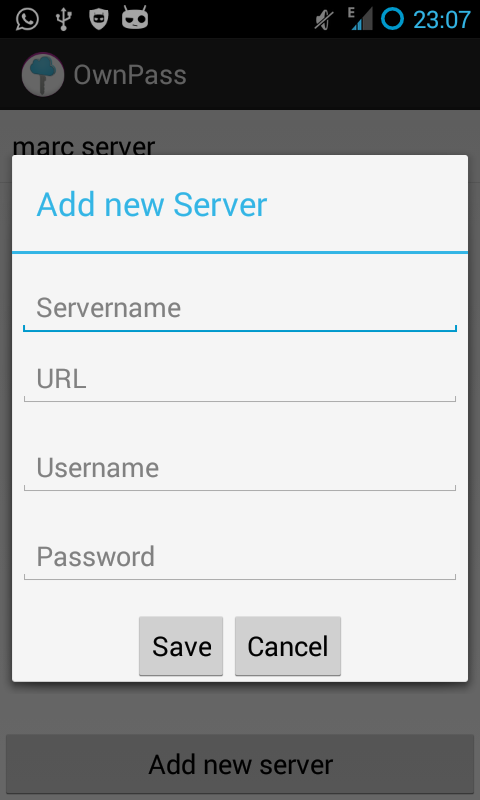
\includegraphics[height=6cm]{screenshots/add_server}
	    \lfig{screenshot-add-server}   
	}
	\hfill
	\subfigure[Dialog to select a server and login]{
	    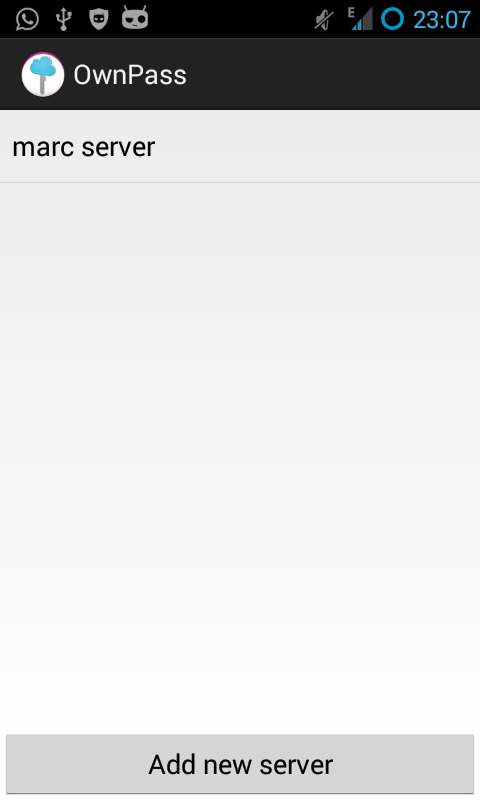
\includegraphics[height=6cm]{screenshots/login}
	    \lfig{screenshot-login}
	}
	\caption{The SigninActivity where one can add, modfiy and delete servers and also connect to an already added server.}
\end{figure}

\begin{figure}
	\centering
	\subfigure[The password list]{
	    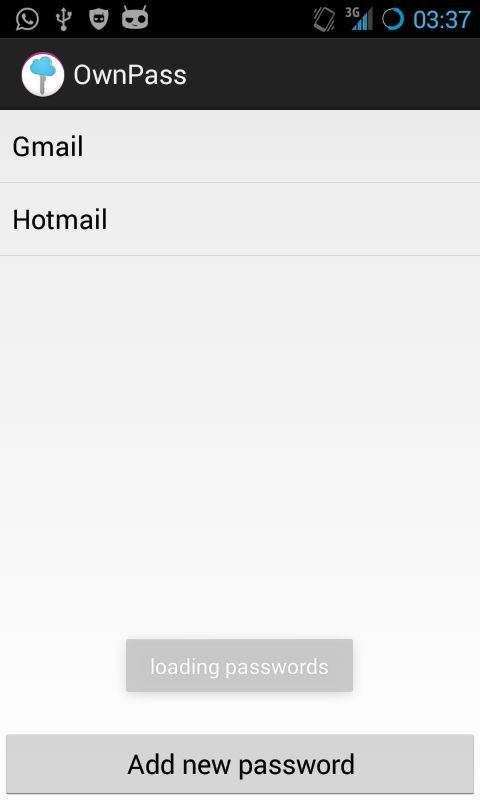
\includegraphics[height=6cm]{screenshots/password_activity}
	    \lfig{screenshot-password-activity}   
	}
\end{figure}

In the same vain that we developed the rest of the application, we also tried to keep the interface as simple and clean as possible. Therefore it consists of only two activities.

The first of these is the SigninActivity that serves to display stored servers and add, edit and delete servers. It can be seen in figures 1(a) and 1(b). This information is stored in the SQLite database to allow us to later query the same information again. A simple click on an existing server tries to connect to that server and transmits the user data. If the login was successful the PasswordManagerActivity is started.

The second activity is the PasswordManagerActivity that displays saved passwords and allows the user to add, modify and delete passwords. Again it uses the SQLite database to cache all passwords to allow a user to access his passwords, even if he does not have any data connectivity.

\section{Implementation}
We created a Server and a Client application. The server is supposed to run on a computer.

The application starts with a ListView of registered servers. The User may decide on which account he wants to store his passwords by just clicking on a server. This will lead to a list of all here  stored passwords. In Both Activities, it's basically the same for servers and for passwords, the User can push the Add button and create a new Object. if he clicks on a particular object for some time a field appears where this object can be deleted or edited. 

We store all the informations about Servers and Passwords on the client side in a class called Database. It creates two tables servers.db and passwords.db with the following properties:

\lstset{language=SQL,frame=ltrb,framesep=5pt,basicstyle=\normalsize,
	 keywordstyle=\ttfamily\color{green},
     identifierstyle=\ttfamily\color{blue}\bfseries,
     commentstyle=\color{black},
     stringstyle=\ttfamily,
     showstringspaces=ture}
\begin{lstlisting}     
 CREATE TABLE servers ( 
         id INTEGER PRIMARY KEY AUTOINCREMENT, 
         name TEXT NOT NULL, 
         url TEXT NOT NULL, 
         username TEXT NOT NULL, 
         password TEXT NOT NULL ) 
\end{lstlisting}
\begin{lstlisting} 	
 CREATE TABLE passwords (
        id INTEGER PRIMARY KEY AUTOINCREMENT,
        server_id INTEGER KEY,
        server_password_id INTEGER KEY, 
        title TEXT NOT NULL,
        url 	TEXT NOT NULL,
        username BLOB NOT NULL,
        password BLOB NOT NULL )
\end{lstlisting}

we use this class Database to store all the informations we will need later on and to handle all the updates. The manipulations like delete, add and edit are created more or less equally.

\subsection{Cryptography}
As we all know that cryptography is hard and a pain, we used the standard Java javax.crypto cryptography library to implement hashing, encryption and decryption.

We decided to use the well known AES symetric encryption cipher in CBC mode and used PKCS5 as the padding scheme:

\lstset{language=Java,caption={SensorWrapper class},label=code} 
\begin{lstlisting}
public Encryption(Server server) {
        ...
        cipher = Cipher.getInstance("AES/CBC/PKCS5Padding");
        ...
    }
    
    ...
    
    public byte[] encrypt(String toEncrypt) {
        ...
        // Generate random IV
        
		...        
        cipher.init(Cipher.ENCRYPT_MODE, key);
        byte[] encryptedString = cipher.doFinal(toEncrypt.getBytes("UTF-8"));
        ...
    }
    ...
}
\end{lstlisting}

At the moment we simply hash the password using the hashing algorithm SHA256 and transfer the hashed password to the server via the REST API. At the same time we use the same hash to de- and encrypt the users usernames and passwords, which of course is a fatal mistake. But for our purposes this suffices, as we do not want anyone to use our system in production yet.

It is important to mention, that we decided to encode all passwords with Base64 to make it easier to debug the connection because of the lack of any binary transfers.

In later implementations, it might be useful to use the bcrypt or scrypt to hash the password to enhance the security of the password hashing algorithm.

\subsection{Problems}
In the following sections we list a few problems we came across while developing the Android application. We did not include any problems we had with the server as this was not the main focus of this project.

\subsubsection{Callbacks}
We wanted to reuse the UserPasswords class to check if a login was successful and also to load all passwords of a user. At first we thought that this was only achievable using some kind of inheritance, but we had the brilliant idea to simply create a UserPasswordCallback interface like this:
\lstset{language=Java,caption={UserPasswordCallback interface},label=code} 
\begin{lstlisting}
public interface UserPasswordCallback {
    public void onSuccess(List<Password> passwordList);
    public void onError(Exception exception);
}
\end{lstlisting}

We implement this interface in both of our activities to allow the UserPasswords AsyncTask to call the onSuccess and onError methods in the postExecute method. This allows us to react differently on errors in both classes as an invalid login should not allow the user to proceed to the PasswordManagerActivity but at the same time should not remove the cached passwords in the PasswordManagerActivity.

\subsubsection{Long clicks}
Because we decided to show the modification dialog of a server and password after a long click on the ListView item, we had to add an onItemLongClickListener to both ListViews. At first we forgot to return true in the called onItemLongClick method which results in the standard onItemClickListener to be called. That does not result in showing the modification dialog but also in signing in which is highly undesirable.

\subsubsection{Inefficiency}
Every time we login to the server we update our local database by 
dropping the current password table and adding all the passwords we get from the server. It's obvious that we reinsert most of the entries. This concept works fine as long as there are just a few password. But consider the case we have some thousand ones we might get an unacceptable latency. It would take much to much time especially for displaying the entries. 

One possible solution would be to send just the information that is needed. But this approach would make the whole application design much more complicated especially for implementing the server. It would have to keep track of which client got which information by now.

\subsubsection{Temporary Loss of Consistency}
The Basic Strategy for changing our database works in a best effort like manner. We update our local database every time when we're adding, deleting or editing a password. On the other hand the server database will only be updated if it's possible to get a connection. If that's not the case we don't do much more at moment.
Consider the case someone makes any changes while he's offline. The Server will never get updated and hence the other affiliated devices will never learn about the modifications. It's even worse because every time the application restarts the local database gets overwritten and all changes will be lost. As the only good side effect we get that the consistency is reestablished.

To solve this problem we would have to add another table that stores informations about all the modifications that couldn't be sent to the server for any reasons. When a connection succeeded it should exchange as much data as possible. In the optimal case both databases get consistent. Otherwise keep the not yet sent passwords stored. 

\subsubsection{Cryptography}
As already mentioned several times through the report, we decided to concentrate on the Android application and did not spend too much time on the cryptographic aspects of our system. For example we know, that it is moronic to send the user's master password in cleartext / to send the same password we use to de- and encrypt usernames and passwords to the server.

We simply did not have the time to acquire the knowledge to inform ourselves, how possible competitors solve this problem and to come up with an improved solution.

\section{Further Plans}
We intended to build some extra features. For example, we wanted to give the client the possibility to save some comments for each Password. Those could be shared among the different devices or just stored locally. 
we also planed to give the clients the possibility not just to register for given Accounts but to create new ones as well. This would be handy if someone wants to share the service with different peoples he didn't even met yet. With our current solution we would have to create for example a website to get the same functionality.
Even though that's much less handy.

A small gimmick we wanted to include is a password and user name  generator. We have even written most of the code but we decided to focus on the main features. 

Something else fairly simple to implement is to provide a button that gives the user the possibility to decide whether it should update the passwords or not.  

\subsection{More Features}
It might be interesting to give the users the possibility to merge the informations of several servers. The simplest approach is to just store all the date on just one server. An other idea would be to let the passwords where they're stored but to create for the user an illusion of storing everything on just one server. It's even possible to store the passwords on several servers to guarantee that no information is lost. The User wouldn't have to remember any longer where what Password is stored.

There are much more Features one might implement, for example some kind of hierarchy between the passwords or to give permissions to other users to access just some specified passwords. But most of them are kind of tricky to implement.

\section{Conclusion}
For the project we could use much of the material we learned in the distributed systems class. Building a Server and a client and let them exchange data is a task in which the benefits of the exercises from the first part clearly appeared. 

When we decided what kind of project we would like to do, we knew that it should be something handy. Something that can be used after we the course ended and we are convinced that our project satisfies this goal. Of course there's still a lot of work that could be done but the main functionalities one might want are implemented. The application can be used now for private purposes.

Overall this project was a fun thing to do. 

% The following two commands are all you need in the
% initial runs of your .tex file to
% produce the bibliography for the citations in your paper.
\bibliographystyle{abbrv}
\bibliography{report}  % sigproc.bib is the name of the Bibliography in this case
% You must have a proper ".bib" file

%\balancecolumns % GM June 2007

\end{document}
